\section{CSO as sources of UHECRs and neutrinos}
\subsection{Magnetic field strength}
%In order to estimate magnetic field strength one outlines two methods in section \ref{sec:equipartition} and \ref{sec:SSA}. Now one only needs to collect data. Of the two methods, the equipartition method is the most reliable and the easiest to collect data for, but uses the assumtion of equipartition, and assumption that is not necessarly the case. The SSA method is more difficult to obtain data for, due to the necessatiy of collecting data at the correct frequency, but does not need an assumption between the magnetic field strength and the energy density of the particles. In addition to this both values will work as great cross checks for different parameters in the system. For Synchrotron self absorption(SSA) $B \propto R^{4}$, while for equipartition $B \propto R^{-2/7}$.

%From table \ref{tab:CSO_sources} one is given the turnover frequency and its corresponding flux density. The problem here is that this value is for the entire source and not any hotspot or lobe. In order to derive the appropriate value one needs to know the size of a lobe, and importantly the fraction of emitted radiation that stem from that lobe compared to the rest of the source. This is a difficult task ridden with selection bias, but one will make an effort to estimate the magnetic field strength. In order to estimate both the SSA and equipartition magnetic field one will turn to a catalogue of 374 strong flat spectrum radio sources, called The VSOP 5 GHz Continuum Survey: The Pre-launch VLBA Observations, \cite{nrao1996}. This catalogue measured high resolution radio images of some  sources contained in table \ref*{tab:CSO_sources} at $5$GHz. These images will allow us to estimate the size of an individual lobe, here we chose the most powerful lobe, and the fraction of the total flux density that comes from this lobe. The same fraction will then be applied to the turnover flux density given in table \ref{tab:CSO_sources} to estimate the turnover flux density from this lobe. Additionally, the NRAO catalogue gives also flux densities measured at $5$GHz allowing us to estimate the equipartition magnetic field strength based on an assumption of the spectral index. One finds an overlap of $10$ sources between the two catalogues, and the extracted values can be found in table \ref{tab:CSO_B}.

In order to estimate magnetic field strength, one outlines two methods in section \ref{sec:equipartition} and \ref{sec:SSA}. Now one only needs to collect data. Of the two methods, the equipartition method is the most reliable and the easiest to collect data for, but uses the assumption of equipartition, an assumption that is not necessarily the case. The SSA method is more difficult to obtain data for, due to the necessity of collecting data at the correct frequency, but does not need an assumption between the magnetic field strength and the energy density of the particles. In addition to this, both values will work as great cross-checks for different parameters in the system. For Synchrotron Self-Absorption (SSA) $B \propto R^{4}$, while for equipartition $B \propto R^{-2/7}$.

From table \ref{tab:CSO_sources} one is given the turnover frequency and its corresponding flux density. The problem here is that this value is for the entire source and not any hotspot or lobe. In order to derive the appropriate value, one needs to know the size of a lobe, and importantly the fraction of emitted radiation that stems from that lobe compared to the rest of the source. This is a difficult task ridden with selection bias, but one will make an effort to estimate the magnetic field strength. In order to estimate both the SSA and equipartition magnetic fields, one will turn to a catalogue of 374 strong flat spectrum radio sources, called The VSOP 5 GHz Continuum Survey: The Pre-launch VLBA Observations, \cite{nrao1996}. This catalogue measured high-resolution radio images of some sources contained in table \ref*{tab:CSO_sources} at $5$GHz. These images will allow us to estimate the size of an individual lobe, here we chose the most powerful lobe, and the fraction of the total flux density that comes from this lobe. The same fraction will then be applied to the turnover flux density given in table \ref{tab:CSO_sources} to estimate the turnover flux density from this lobe. Additionally, the NRAO catalogue also gives flux densities measured at $5$GHz, allowing us to estimate the equipartition magnetic field strength based on an assumption of the spectral index. One finds an overlap of $10$ sources between the two catalogues, and the extracted values can be found in table \ref{tab:CSO_B}.


\begin{table}
    \centering
    \begin{tabular}{|c|c|c|c|c|c|c|c|}
    \hline
    \textbf{Name} & \textbf{z} & \textbf{Class} & \textbf{$\nu_t$} & \textbf{$S_{\nu_t}$} & \textbf{$\nu_{5GHz}$} & \textbf{$\theta_{lobe}$} & \textbf{$S_{\nu_{5GHz}}$} \\
    \hline
    J0029+345 & 0.517 & 2.0 & 0.8 & 1.178 & 5 & 2.1 & 0.766 \\
    J0111+3906 & 0.66847 & 2.0 & 4.0 & 0.88189 & 5 & 0.95 & 0.862 \\
    J0119+3210 & 0.0602 & 2.2 & 0.4 & 0.5125 & 5 & 9.85 & 0.205 \\
    J0405+3803 & 0.055 & 2.0 & 0.07 & 2.554 & 5 & 2.7 & 0.418 \\
    J0713+4349 & 0.518 & 2.0 & 1.9 & 0.94311 & 5 & 1.45 & 0.722 \\
    J1035+5628 & 0.0460 & 2.0 & 1.3 & 1.0659 & 5 & 1.6 & 0.741 \\
    J1158+2450 & 0.203 & 2.2 & 2 & 0.588 & 5 & 4 & 0.566 \\
    J1347+1217 & 0.121 & 2.2 & 0.4 & 1.3947 & 5 & 1 & 0.488 \\
    J1407+2827 & 0.077 & 2.1 & 4.9 & 2.9375 & 5 & 1.2 & 2.350 \\
    J2022+6136 & 0.2266 & 2.1 & 4.086 & 1.57256 & 5 & 2 & 1.787 \\
    J2355+4950 & 0.238 & 2.2 & 0.7 & 1.5450 & 5 & 1.8 & 0.791 \\
    \hline
    \end{tabular}
    \caption{Overlapping sources between the NRAO catalogue and \cite{kiehlmann2023compact} and the extracted values scaled to represent one lobe hotspot.}
    \label{tab:CSO_B}
\end{table}

From here one can estimate the magnetic fields via both methods. 

\begin{figure}
    \centering
    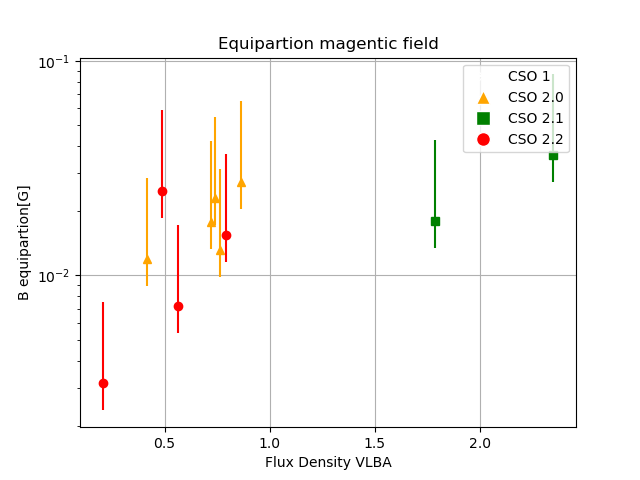
\includegraphics[width=0.8\textwidth]{C:/Users/henri/OneDrive/Documents/NTNU/Semester 10/Masteroppgave/Plots/Equipartion.png}
    \caption{Magnetic field strength estimated from the equipartition method. The errobars are calculated from the span of values obtained from different spectral index ranging from $0.6$ to $1.3$.}
    \label{fig:B_field}
\end{figure}

\begin{figure}
    \centering
    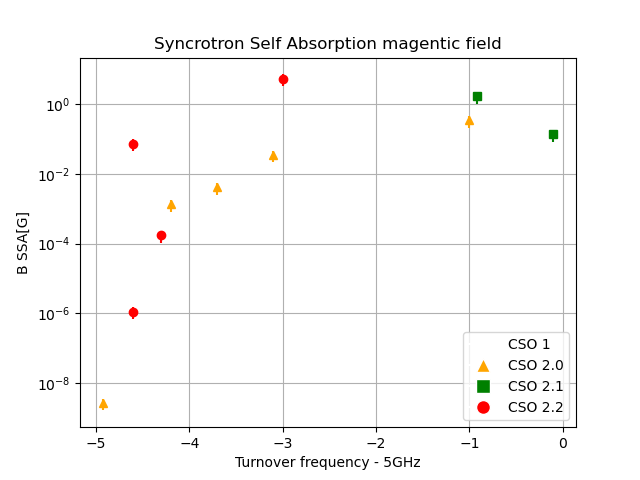
\includegraphics[width=0.8\textwidth]{C:/Users/henri/OneDrive/Documents/NTNU/Semester 10/Masteroppgave/Plots/SSA.png}
    \caption{Magnetic field strength estimated from the SSA method. The errobars are calculated from the span of values of $b(\alpha)$ obtained from different optical thickness. $b(\alpha)$ ranges from $1.08$ to $2.38$.}
    \label{fig:B_field_SSA}
\end{figure}

%The result of the magnetic field estimations are a little varied, but the most reliable numbers is a magnetic fields strenght between $5 \times 10^{-3}$ and $1 \times 10^{-1}$ G. Here one relies most heavilly on the equipartition argument due to the SSA estimation being very biased, as the estimation of the lobe size is wrong for turnover frequencies lower than the imaging. The lobe size estimation is based on the images from the $5$ GHs survey, and as one sees in figure \ref{fig:B_field_SSA} the magnetic field strenght from SSA calculations is heavilly dependent on the different between the turnover frequency and the frequency of the observation. The SSA still give values for the magnetic field strength that are in the same order of magnitude as the equipartition method at turnover frequencies closer to the measured frequency and even go above.

%The equipartition calculations is also greatly affected by the choice of spectral index, as seen by the large errorbars, but places the sources neatly in the same order of magnitude as the best SSA calculations. For SSA calculations that go above the equipartition values one can have several explinations. Firstly it could be that the equipartition argument does not hold and that the magnetic field is stronger than the equipartition value, this can be investigated by looking at jet power. Secondly it could be that there are other factors than synchrotron self absorption that make the source optically dense. If one includes free-free absorption one could shift the turnover frequency to a higher value, resulting in a higher magnetic field measurement. This is not investigated in this work, but is a possible explanation for the high magnetic field strength. For the continued work in this thesis one will use the equipartition magnetic field strength as the most reliable value, but will also consider the SSA magnetic field strength as a possible value. The general magnetic field of a CSO in all classes would then be $B = 10^{-2}$ G. 

%The estimation of the radius of our emitting regions in the previous section can be put under question. In order the estimate the precise value of our emitting regions one would idealy measure the flux at the turnover frequency in order for the most flux not to drop under the sensitivity of the telescope. Even given this \cite{1983ApJ...264..296M} would estimate the angular size of the source is still $\theta_{\text{true}} = 1.8\times \theta_{\text{FWHM}}$. For some sources in table \ref{tab:CSO_B} one measures close to the turnover frequency, but for most a more thorough consideration could be in order. The equipartition method is not as sensitive to the size of the source, but one should still be careful not taking the values at face value.

%In order to do so, another method of estimating the radius of our lobes is outlined in \cite{W_jtowicz_2020}. They uses a relation between the total linear size of an objects and the estimated relations between the semi-major axis and the semi-minor axis. The argument is that CSOs have relativly large aspect rations between their axis, with an estimation equaling $b/a \approx 0.25$. From this they introduce the effective radius of the radio lobes via 


The result of the magnetic field estimations is a little varied, but the most reliable numbers indicate a magnetic field strength between $5 \times 10^{-3}$ and $1 \times 10^{-1}$ G. Here, one relies most heavily on the equipartition argument due to the SSA estimation being very biased, as the estimation of the lobe size is wrong for turnover frequencies lower than the imaging. The lobe size estimation is based on the images from the $5$ GHz survey, and as one sees in figure \ref{fig:B_field_SSA}, the magnetic field strength from SSA calculations is heavily dependent on the difference between the turnover frequency and the frequency of the observation. The SSA still gives values for the magnetic field strength that are in the same order of magnitude as the equipartition method at turnover frequencies closer to the measured frequency and even go above.

The equipartition calculations are also greatly affected by the choice of spectral index, as seen by the large error bars, but place the sources neatly in the same order of magnitude as the best SSA calculations. For SSA calculations that go above the equipartition values, one can have several explanations. Firstly, it could be that the equipartition argument does not hold and that the magnetic field is stronger than the equipartition value; this can be investigated by looking at jet power. Secondly, it could be that there are other factors than synchrotron self-absorption that make the source optically dense. If one includes free-free absorption, one could shift the turnover frequency to a higher value, resulting in a higher magnetic field measurement. This is not investigated in this work but is a possible explanation for the high magnetic field strength. For the continued work in this thesis, one will use the equipartition magnetic field strength as a reliable lower value but will also consider the SSA magnetic field strength as a possible value. %The general magnetic field of a CSO in all classes would then be $B = 10^{-2}$ G.

The estimation of the radius of our emitting regions in the previous section can be put under question. In order to estimate the precise value of our emitting regions, one would ideally measure the flux at the turnover frequency in order for the most flux not to drop under the sensitivity of the telescope. Even given this, \cite{1983ApJ...264..296M} would estimate the angular size of the source is still $\theta_{\text{true}} = 1.8\times \theta_{\text{FWHM}}$. For some sources in table \ref{tab:CSO_B}, one measures close to the turnover frequency, but for most, a more thorough consideration could be in order. The equipartition method is not as sensitive to the size of the source, but one should still be careful not to take the values at face value. 

The biggest problem with SSA method for lower turnover frequencies is that one might underestimate 


%with this estimation one can estimate the size of the lobes for the sources in table \ref{tab:CSO_B}, and compare the resulting values to the radii obtained from the FWHM of the images in the NRAO catalogue.  here one will note that this is an estimation of lobe size and not necessarly the hotspot which we are interested in. The results 



%\subsection{Energy budget}
%Via the energy budget of the CSOs, one can get an idea of where it is possible to accelerate protons to UHECR energies. The most natural place is in the Hillas diagram, where one can compare the size and magnetic field strength of the system to the maximum energy of the proton. From our magnetic field estimations one can see that the magnetic field strength is between $10^{-2}$ and $1$ G. The radius of our emitting region is from the order of $2$ pc to $10$ pc when the lobe expands. It would be reasonable to assume that as the lobe expands the magnetic field strength decreases, but as it expands more energy is also being fed into the hot spots, therefore one will could assume a magnetic field strength of $10^{-1}$ G for the biggest lobes as well. The choice of magnetic field strength and radius of the emitting region can be compared to other candidates for emitters and is shown in figure \ref{fig:Hillas}.
With this estimation, one can estimate the size of the lobes for the sources in table \ref{tab:CSO_B}, and compare the resulting values to the radii obtained from the FWHM of the images in the NRAO catalogue. Here, one will note that this is an estimation of lobe size and not necessarily the hotspot which we are interested in. The results...

\subsection{Energy budget}
Via the energy budget of the CSOs, one can get an idea of where it is possible to accelerate protons to UHECR energies. The most natural place is in the Hillas diagram, where one can compare the size and magnetic field strength of the system to the maximum energy of the proton. From our magnetic field estimations, one can see that the magnetic field strength is between $10^{-2}$ and $1$ G. The radius of our emitting region is on the order of $2$ pc to $10$ pc when the lobe expands. It would be reasonable to assume that as the lobe expands, the magnetic field strength decreases, but as it expands, more energy is also being fed into the hotspots. Therefore, one could assume a magnetic field strength of $10^{-1}$ G for the biggest lobes as well. The choice of magnetic field strength and radius of the emitting region can be compared to other candidates for emitters and is shown in figure \ref{fig:Hillas}.


\begin{figure}
    \centering
    \includegraphics[width=0.8\textwidth]{C:/Users/henri/OneDrive/Documents/NTNU/Semester 10/Masteroppgave/Plots/hillas.png}
    \caption{Hillas diagram for the CSO. The red line represents the maximum energy of the proton that can be accelerated in the system, and blue is the same just for Iron. }
    \label{fig:Hillas}
\end{figure}

%From the figure it becomes clearer that CSO is a class worthy of being investigated further, both their lobe size, and their magnetic field strength make them great candidates. As for all potential sources one observes one needs a highly efficient acceleration mechanism in order to accelerate the protons. The efficiency of acceleration is described by the $\beta$ factor in figure \ref*{fig:Hillas}. The CSO hotspots separate themselves from usual AGN hotspots which are attributed to large lobes at the end of the jet in huge radio galaxies. The more compact hotspots in CSOs might be more efficient in accelerating protons, but this needs to be looked into further.  
\subsubsection{x-ray power}
%In stduies such as \cite{Jacobsen:2015mga} and \cite{10.1111/j.1745-3933.2008.00499.x} one discuss the possibility of using the x-ray flux or hard x-ray flux as a proxy for hadronic acceleration. This is a common start in trying to probe the biggest emitters of neutrinoes and UHECRs, and it is worth looking at CSOs this way as well. The biggest caveat with this method is that one usually attributes the x-ray flux to the core region, and then one might have different mechanisms for acceleration than one has in the hotspots. In the case of our model of a CSO SED one immeditly sees that the total x-ray flux from the x-ray corona will be a factor of the total accretion luminosity. For our model of timescales later in the chapter one assumes the fraction to be $f_X = 0.3$. and for this one recived a typical total x-ray corona flux of $3 \times 10^{42} $erg/s. This number is quite a lot higher than  what was found by  \cite{bronzini2024investigating} who using two spectral models, found a x-ray flux for two compact sources, PKS 1718-649 and TXS 1146+596, to be just shy of $10^{41}$ erg/s. In addition to this estimate \cite{W_jtowicz_2020} cites the x-ray flux of 17 CSOs and here one will do another cross correlation with the CSOs in table \ref*{tab:CSO_sources}. The results can be seen in table \ref{tab:CSO_xray}.
From the figure, it becomes clearer that CSOs are a class worthy of being investigated further; both their lobe size and their magnetic field strength make them great candidates. As with all potential sources, one observes that a highly efficient acceleration mechanism is needed to accelerate the protons. The efficiency of acceleration is described by the $\beta$ factor in figure \ref*{fig:Hillas}. The CSO hotspots separate themselves from usual AGN hotspots, which are attributed to large lobes at the end of the jet in huge radio galaxies. The more compact hotspots in CSOs might be more efficient in accelerating protons, but this needs to be looked into further.

\subsubsection{X-ray power}
In studies such as \cite{Jacobsen:2015mga} and \cite{10.1111/j.1745-3933.2008.00499.x}, one discusses the possibility of using the X-ray flux or hard X-ray flux as a proxy for hadronic acceleration. This is a common start in trying to probe the biggest emitters of neutrinos and UHECRs, and it is worth looking at CSOs this way as well. The biggest caveat with this method is that one usually attributes the X-ray flux to the core region, and then one might have different mechanisms for acceleration than one has in the hotspots. In the case of our model of a CSO SED, one immediately sees that the total X-ray flux from the X-ray corona will be a factor of the total accretion luminosity. For our model of timescales later in the chapter, one assumes the fraction to be $f_X = 0.3$, and for this, one received a typical total X-ray corona flux of $3 \times 10^{42}$ erg/s. This number is quite a lot higher than what was found by \cite{bronzini2024investigating}, who, using two spectral models, found an X-ray flux for two compact sources, PKS 1718-649 and TXS 1146+596, to be just shy of $10^{41}$ erg/s. In addition to this estimate, \cite{W_jtowicz_2020} cites the X-ray flux of 17 CSOs, and here one will do another cross-correlation with the CSOs in table \ref*{tab:CSO_sources}. The results can be seen in table \ref{tab:CSO_xray}.


\begin{table}
    \centering
    \begin{tabular}{|c|c|c|c|}
        \hline
        \textbf{Name} & \textbf{z} & \textbf{Class} &   \textbf{$L_{\text{X-ray}}$} \\
        \hline

        

        J0111+3906 & 0.66847 & 2.0 & 70 \\
        J0119+3210 & 0.0602 & 2.2 & $<$1.0 \\
        J0713+4349 & 0.518 & 2.0 & 394 \\
        J1511+0518 & 0.084 & 2.0 & 30 \\
        J1939-6342 & 0.183 & 2.0 & 6 \\
        J1944+5448 & 0.263 & 2.0 & 7.31 \\
        J1945+7055 & 0.101 & 2.2 & 12 \\ 
        J2022+6136& 0.227 & 2.1 & 112 \\
        J2355+4950 & 0.238 & 2.2 & 13 \\
        \hline
    \end{tabular}
    \caption{X-ray flux of the CSOs in table \ref{tab:CSO_sources} found in the data set in \cite{W_jtowicz_2020}. The X-flux is given in units of $10^{42}$ erg/s.}
\label{tab:CSO_xray}
\end{table}

%After cross correlation one is left with $9$ objects that are in both catalogues. The X-ray flux of these objects span the range between $6-394 \times 10^{42}$ erg/s for CSO $2.0$ which has the most data. CSO 2.2 with three data points does not have any that exceed $13 \times 10 ^{42}$ erg/s and the lone CSO $2.1$ sits at a powerful $112\times 10^{42}$erg/s. With these values one can compare them to other jetted AGN like Bl lacs and blazars. One will do this by looking at the total x-ray emissivity of the sources and compare it to the local emissivity of the UHECRs. The total x-ray emissivity is given by $Q_{\text{X-ray}} = L_{\text{X-ray}} n_{\text{CSO}}$. The results can be seen in figure \ref{fig:X-ray_em}. The amount of data collect is very low and one can not make any strong conclusions from this, but using the values as a benchmark value one can see that the x-ray emissivity of the CSO $2.0$ and $2.1$ span a sizeable area above the local emissivity of UHECRs and neutrinos.  CSO $2.2$ seem to emit X-ray at a lower rate but still powerful enough to exceed the local emissivity of UHECRs. In previous work I have found that even though the X-ray flux is a good indicator of relativisitc particles, in most cases electrons, there still is work to be done relating it to UHECRs and neutrino. Given that the X-ray flux of the CSOs surpass the local emissivity of UHECRs and neutrinos significantly one can say that the CSOs are also good candidates for UHECRs and neutrino production when compared to other AGN. 

After cross-correlation, one is left with $9$ objects that are in both catalogues. The X-ray flux of these objects spans the range between $6-394 \times 10^{42}$ erg/s for CSO $2.0$, which has the most data. CSO 2.2, with three data points, does not have any that exceed $13 \times 10^{42}$ erg/s, and the lone CSO $2.1$ sits at a powerful $112 \times 10^{42}$ erg/s. With these values, one can compare them to other jetted AGN like BL Lacs and blazars. One will do this by looking at the total X-ray emissivity of the sources and comparing it to the local emissivity of the UHECRs. The total X-ray emissivity is given by $Q_{\text{X-ray}} = L_{\text{X-ray}} n_{\text{CSO}}$. The results can be seen in figure \ref{fig:X-ray_em}. 

The amount of data collected is very low, and one cannot make any strong conclusions from this, but using the values as a benchmark, one can see that the X-ray emissivity of the CSO $2.0$ and $2.1$ spans a sizeable area above the local emissivity of UHECRs and neutrinos. CSO $2.2$ seems to emit X-ray at a lower rate but still powerful enough to exceed the local emissivity of UHECRs. In previous work, I have found that even though the X-ray flux is a good indicator of relativistic particles, in most cases electrons, there still is work to be done relating it to UHECRs and neutrinos. Given that the X-ray flux of the CSOs surpasses the local emissivity of UHECRs and neutrinos significantly, one can say that the CSOs are also good candidates for UHECRs and neutrino production when compared to other AGN.



\begin{figure}[ht]
    \centering
    \begin{subfigure}[b]{0.49\textwidth}
        \centering
        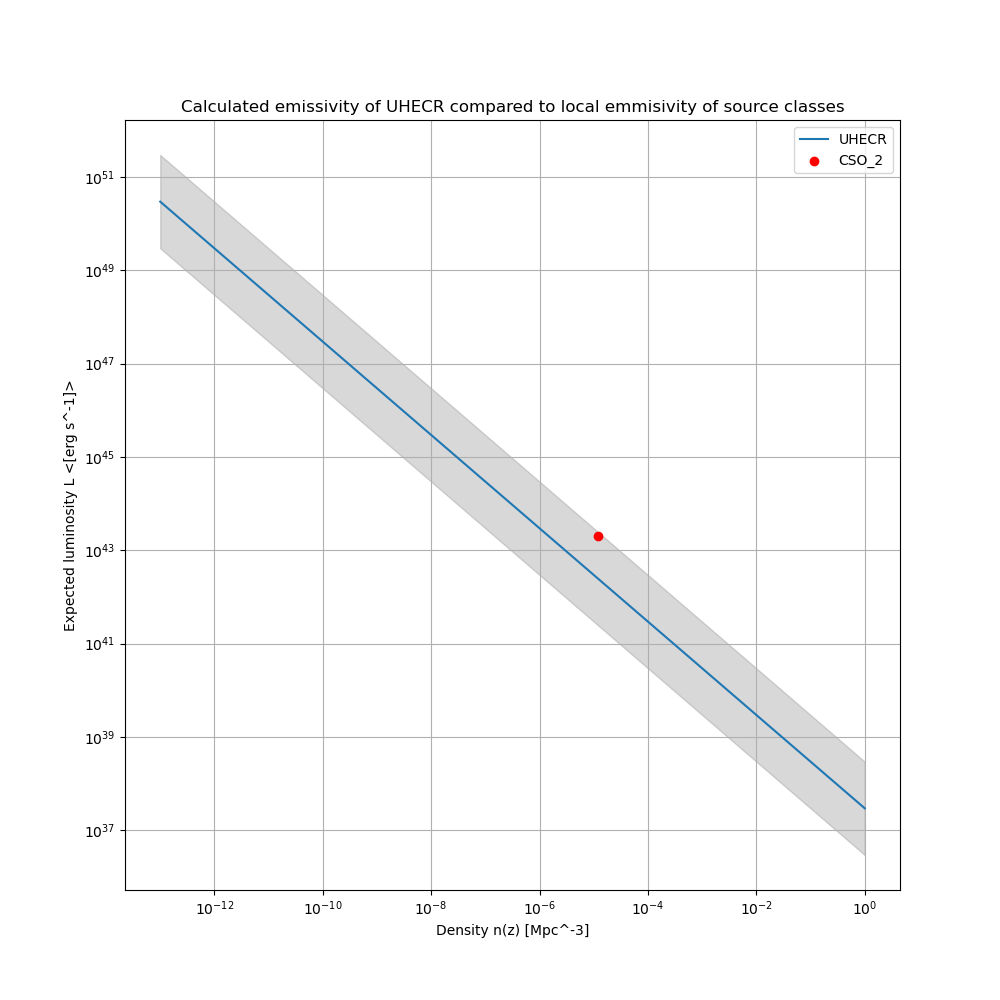
\includegraphics[width=\textwidth]{C:/Users/henri/OneDrive/Documents/NTNU/Semester 10/Masteroppgave/Plots/L_n_uhecr_calc_cso.png}
        \caption{UHECRs emissivity compared to X-ray luminosity of 
        AGN classes }
        \label{fig:uhecr_em}
    \end{subfigure}
    \hfill
    \begin{subfigure}[b]{0.49\textwidth}
        \centering
        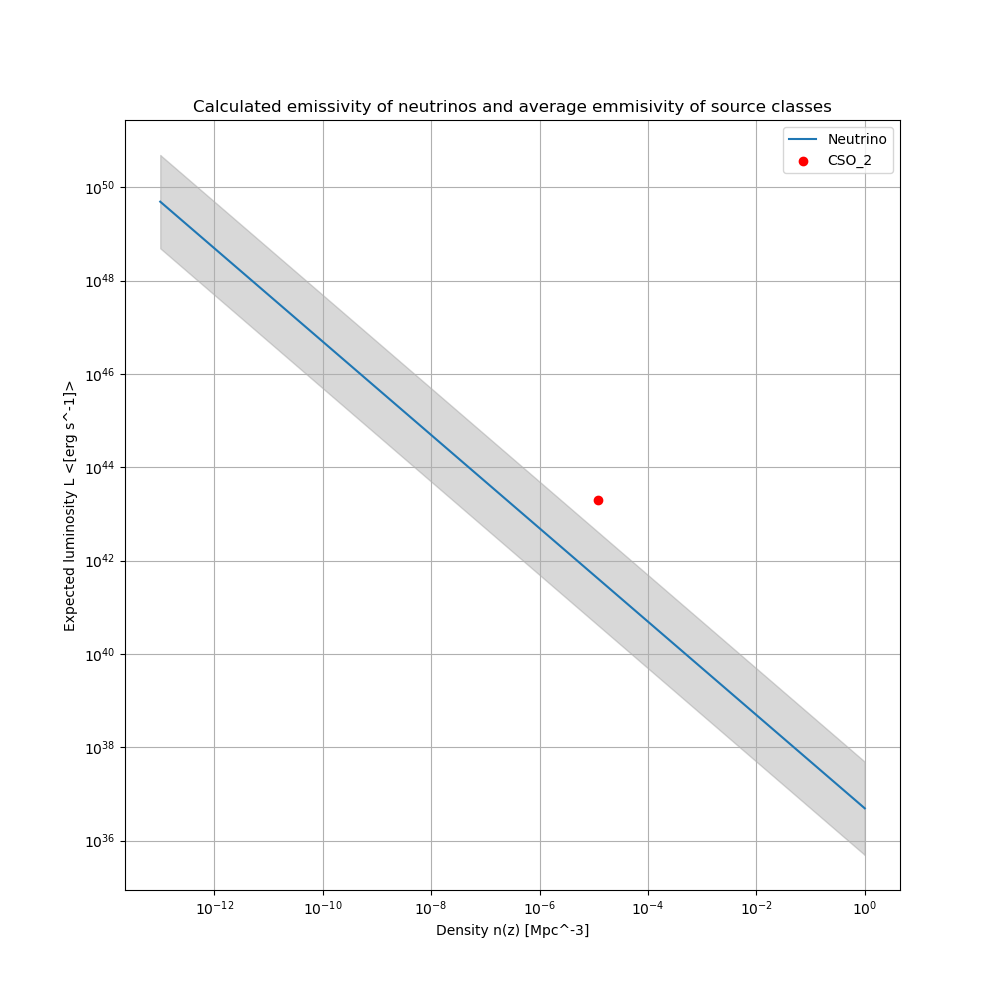
\includegraphics[width=\textwidth]{C:/Users/henri/OneDrive/Documents/NTNU/Semester 10/Masteroppgave/Plots/L_n_neut_calc_cso.png}
        \caption{Neutrinos emissivity compared to X-ray luminosity of AGN classes}
        \label{fig:neut_em}
    \end{subfigure}
    %\caption{Neutrinos emissivity compared to X-ray luminosity of CSO classes }
    \label{fig:X-ray_em}
\end{figure}


\subsubsection{Radio power}



\subsubsection{Jet power}
%The jet power of jetted AGN can be an important parameter in constraining parameters such as particle energy density, and as one will argue if one can move away from equipartition. If the jet energy is carried by particles one can relate the comoving particle density to the stationary frame jet power $P_j$ as, 



%This is for a two sided jet, where $\Omega_j$ is the jet opening angle in sr. The jet power relation here includes the assumption that the jet is carried by electrons, and that the jet power is related to the bulk Lorentz factor of the plasma outflow. By using a general particle distribution for electrons for example as seen in equation \ref{eq:proton_spectrum} and including a factor to account for kinetic energy being carried by protons one can represent the jet power as a function of the kinetic energy carried by particles. One adds to this the power required to expel magnetic field laden plasma given as



%By now including the equipartion magnetic field $B_{\text{eq}}$ and rewriting the kinetic terms as done in section \ref{sec:equipartition}  one can relate the minimum jet power as a function of the equipartion magnetic field. One is skipping a few steps of derivation, but this can be found in \cite{BHradiation} on page 136. The result is the minimum jet power of the system as a function of the equipartition magnetic field strength given as

The jet power of jetted AGN can be an important parameter in constraining parameters such as particle energy density, and as one will argue, if one can move away from equipartition. If the jet energy is carried by particles, one can relate the comoving particle density to the stationary frame jet power $P_j$ as,

\begin{equation}
    \frac{P_j}{2\Omega_j R^2 c \beta (\Gamma m_e c^2)}
\end{equation}

This is for a two-sided jet, where $\Omega_j$ is the jet opening angle in sr. The jet power relation here includes the assumption that the jet is carried by electrons and that the jet power is related to the bulk Lorentz factor of the plasma outflow. By using a general particle distribution for electrons, for example, as seen in equation \ref{eq:proton_spectrum} and including a factor to account for kinetic energy being carried by protons, one can represent the jet power as a function of the kinetic energy carried by particles. One adds to this the power required to expel magnetic field-laden plasma given as

\begin{equation}
    P_b = 2 \frac{B^2}{8\pi} \Omega_j R^2 c \beta \Gamma^2
\end{equation}

By now including the equipartition magnetic field $B_{\text{eq}}$ and rewriting the kinetic terms as done in section \ref{sec:equipartition}, one can relate the minimum jet power as a function of the equipartition magnetic field. One is skipping a few steps of derivation, but this can be found in \cite{BHradiation} on page 136. The result is the minimum jet power of the system as a function of the equipartition magnetic field strength given as

\begin{equation}
    P_j(B_{\text{eq}}) = \frac{14}{3}\pi c \beta \Gamma^2 R^2 \frac{B_{\text{eq}}^2}{8 \pi}
\end{equation}


The last quantities that need to be estimated are the bulk Lorentz factor and, importantly, jet $\beta$, or the speed of expansion into the surrounding medium. The bulk Lorentz factor of our jet is estimated to be $\Gamma < 1.1$ since CSO jets are not relativistically beamed. The last value is the expansion speed of the jet, which will vary from class to class. In the case of CSO $2.0$, one will estimate a value of $\beta$ between $0.1 - 0.4$ c. In \cite{sullivan2024smallscale}, they cite the expansion speed of a CSO $2.0$ to be approximately $200 \times c_s = 200 \times 250$ km/s, where $c_s$ is the sound speed. This gives a value of $\beta = 0.166$ c. Part of the definition of CSO $2.1$ is that the jet is decelerating, and therefore one would expect $\beta$ to lie between $0.1$ and $8\times 10^{-4}$ c. Lastly, the speed of the jet in CSO $2.2$ is by definition extremely low or non-existent, where the apparent motion of emitting bubbles is due to adiabatic expansion. Therefore, one argues that the speed of any emitting blob is to move at the speed of sound in the medium, and therefore $\beta = 8\times 10^{-4}$ c. For values of jet energy derived this way, one will argue that they mostly will work for CSO $2.0$ due to the fact that their jet opening angle has not evolved greatly from their initial state.

One will need to compare this jet power to another method in order to investigate the underlying dynamics. In \cite{Blandford_1977}, one finds a relation between the jet power and the accretion rate of the system. The relation is given as

\begin{equation}
    P_j = k \dot{M} c^2
\end{equation}

where $k$ is a constant that depends on the rotation velocity of the system's black hole. The various values of $k$ range from $0.3$ to $2$, where $k=2$ represents a maximally spinning black hole, $\Omega_{\text{max}} = c^3/2GM$. One can estimate the accretion rate as a fraction of the X-ray luminosity via some simple assumptions. Like our broadband SED modeling, one assumes that the X-ray luminosity is a fraction of our accretion luminosity $L_{\text{X-ray}} = f_X L_{\text{d}}$. The accretion rate is given as $L_{\text{d}} = \eta \dot{M} c^2$ where $\eta$ is the efficiency of the accretion disk. By substituting the mass accretion rate as a function of the X-ray luminosity, one can get a simple estimate for the jet power. The resulting jet power is given as

\begin{equation}
    \label{eq:jet_power}
    P_j = \frac{k}{\eta f_X} L_{\text{X-ray}} = \alpha L_{\text{X-ray}}
\end{equation}

Here, $\alpha$ is a constant that absorbs the other constants since they are most likely dependent on each other. One will utilize the same table as before to estimate the jet power of the CSOs, but one needs to define the equipartition magnetic field for them as well. Since one does not have NRAO data for these sources, one will use the relation between linear size and radius to estimate the radius of the lobes. Otherwise, $S_v$ is given in \cite{W_jtowicz_2020} with the corresponding X-ray luminosity. The jet power can then be seen in figure \ref{fig:jet_power}.


\begin{figure}
    \centering
    \includegraphics[width=0.8\textwidth]{C:/Users/henri/OneDrive/Documents/NTNU/Semester 10/Masteroppgave/Plots/jet_power.png}
    \caption{Jet power of the CSOs in table \ref{tab:CSO_sources}. The jet power is calculated using the minimum jet power argument based on magnetic field equipartition. The bars in line with each line represent the estimated jet power based on the X-ray luminosity varying the value of $\alpha$ in equation \ref{eq:jet_power}.} While the line representing minimum jet power is varying based on $\beta$ values. 
    \label{fig:jet_power}
\end{figure}

It becomes clear that the gap between X-ray flux and CSO $2.2$s is too large to account for the jet power of the system. This is not surprising since all X-ray flux measured is attributed to the core region but this will likely not be the case. As seen in the SED figure \ref{fig:SED_sep} the x-ray flux can have multiple sources, of which upscattering by relativistic electrons happening outside the x-ray corona is very likely. Therefore, this comparisson has some big caveat when it comes to X-ray estimated jet power. On the other hand The minimum jet powers of CSO$2.0$ and $2.1$ are more inline with the power estimated via the X-ray luminosity. This might indicate that more of the x-ray flux from these sources is related to the x-ray core, and our assumption of the x-ray flux being a proxy for jet power is more valid. 


\subsection{Time scales }
Looking at characteristic timescales for CSOs is a powerful tool for understanding the maximum energy that can be obtained from the system. In section 4, one outlined the general method, and here one will present the results for CSO 2s.

With given data obtained from measurements, one will define conservative estimates for an acceleration region in the CSO. The regions of interest are the hotspots created during the CSO 2.0 and 2.1 stages, and one will observe that these are good regions for acceleration. The first constant that needs to be estimated is the size of our emitting system. From observations, it is clear that the radio lobes expand significantly during the CSO lifetime. From radio variations, which are on the order of tens of years, a reasonably conservative estimate for the size of the lobes is $R_{\text{lobe}} = 2$ pc. In addition to this size requirement, one will also include the lifetime of the source, which is on the order of $10^3$ years.

In estimating the magnetic field strength, one found the values of typical lobes to be $B = 10^{-2}$ G from the equipartition argument. This value has been found before in previous literature and is a reasonable lower limit for the magnetic field strength. It is important to note that the magnetic field strength is a very important parameter and yet bears significant uncertainty. It may very well be that the magnetic field strength is higher than this value, and one will discuss this in the following sections.

For the photopion production, one will use the photon field as described in section 4, where the used parameters can be found in table \ref{tab:SED_params}. This field is based on the field of a much larger AGN, but one assumes for this discussion that the field is similar in the CSO. One can compare this generated field to the ones presented in \cite{bronzini2024investigating}, where they find a similar magnitude and shape of the resulting SED. A significant note is that the field is also not strongly beamed, giving room for other parts of AGNs to be seen. The resulting SED is seen in figure \ref{fig:SED_sep}. The exact shape of the SED is not incredibly important for the following discussion, but the broad shape and magnitude are important. The exact shape of the SED will become more important when one starts looking for observational signatures of the acceleration, such as gamma rays, and here one can use the model SED and minimize the parameter space to find the best fit.


\begin{figure}
    \centering
    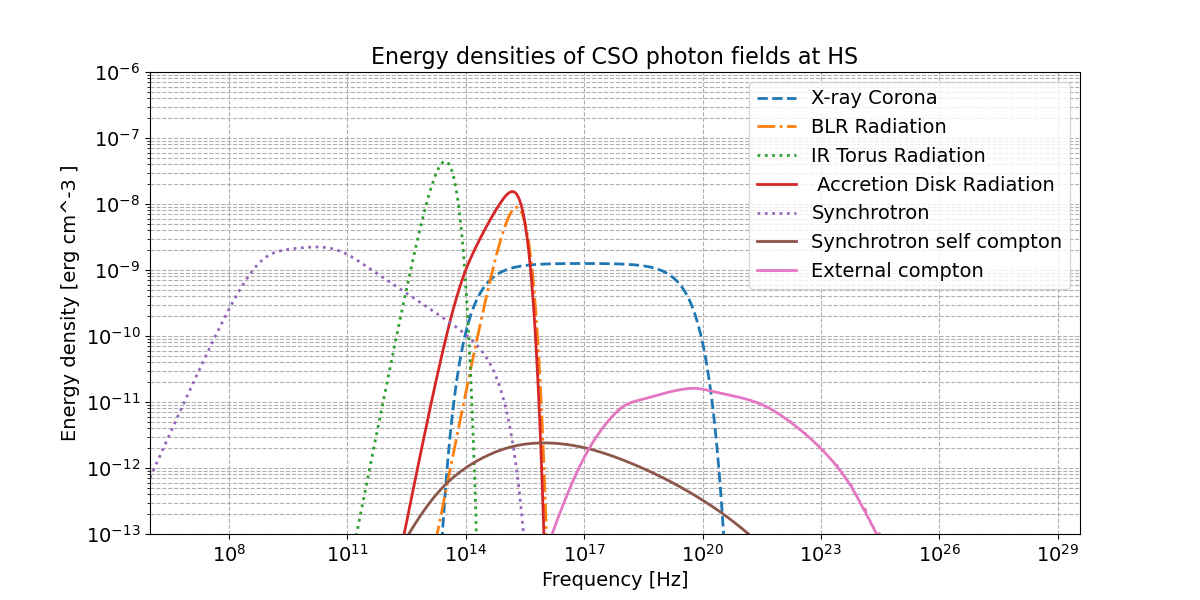
\includegraphics[width=0.8\textwidth]{C:/Users/henri/OneDrive/Documents/NTNU/Semester 10/Masteroppgave/Plots/SEDs_sep.png}
    \caption{SED of the different regions in the CSO. The SED is based on the parameters in table \ref{tab:SED_params}.}
    \label{fig:SED_sep}
\end{figure}





\begin{table}
    \centering
    \begin{tabular}{|c|c|}
        \hline
        Parameter & Value \\
        \hline
        $L_{d}$ & $10^{43}$ erg/s \\
        $GM$ & $G 10^{8} M_{\odot}$ \\
        $RS$ & $\frac{2GM}{c^2}$ \\
        $\eta$ & 0.1 \\
        $f_{X}$ & 0.3 \\
        $R_{X}$ & 30$ RS $\\
        $\beta$ & 0.4 $c$\\
        $f_{\text{BLR}}$ & 0.1 \\
        $R_{\text{BLR}}$ & $10^{17} \sqrt{L_{d}/10^{45}}$ cm \\
        $f_{\text{IR}}$ & 0.5 \\
        $R_{\text{IR}}$ & $2.5 10^{18}\sqrt{L_{d}/10^{45}}$ cm \\
        $\Gamma$ & 1.1 \\
        \hline
    \end{tabular}
    \caption{Parameters used to determine the SED of the different regions.}
    \label{tab:SED_params}
\end{table}


From the above parameters one can estimate the characteristic timescales for the CSO, seen in figure \ref{fig:timescales}. 

\begin{figure}
    \centering
    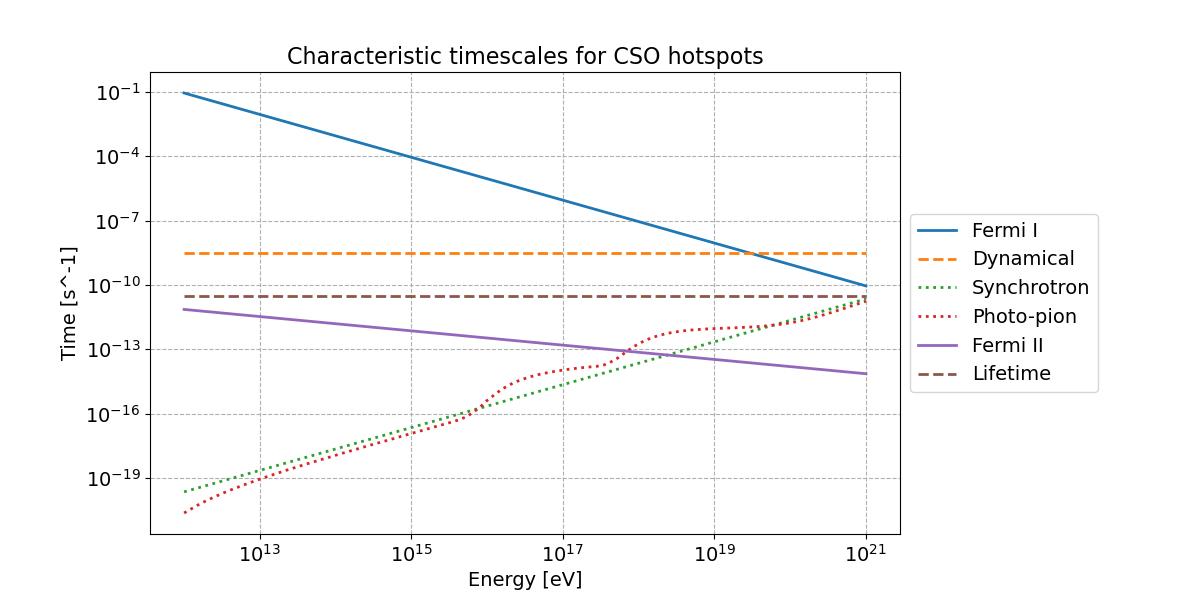
\includegraphics[width=0.8\textwidth]{C:/Users/henri/OneDrive/Documents/NTNU/Semester 10/Masteroppgave/Plots/Time_scales.png}
    \caption{Characteristic timescales for the CSO. Processes included is synchrotron losses and photopion losses. The timescales are calculated for a spherical size of $R_{\text{lobe}} = 2 pc$ and a magnetic field strength of $B = 10^{-2} G$. The photon field is based on the parameters in table \ref{tab:SED_params}.}
    \label{fig:timescales}
\end{figure}
The timescales show us that high-energy protons can, and in any case will, under the right conditions, accelerate up to energies of $<10^{20}$ eV. This limit is capped by the dynamical size of the emitting region and, of course, the magnetic field strength. The timescales also show us that the acceleration is dominated by synchrotron losses and photopion losses, and due to their small value, one would need to consider pair-pair losses as well, which is not done in this analysis. The lack of photopion loss dominance is a good sign for proton acceleration since it has been a limiting factor in other studies such as \cite{peretti2023diffusive}, where one has a higher luminosity object with processes happening even closer to the central engine. One can confirm the lack of photopion by comparing it to the work of \cite{TAKAMI2011749}, which considered a young radio AGN with much bigger lobe sizes and much higher luminosity. In this case, the photopion losses are much higher than the synchrotron losses, and the acceleration is limited by the photopion losses. But one will note that \cite{TAKAMI2011749} did not consider the lifetime of the system, that is to say, the duration for which a CSO could maintain the shock structure that allows for acceleration, which I believe would severely limit the acceleration. The lack of photopion interaction will also be a limiting factor for neutrino production, something that will be discussed in the following sections.


\subsection*{Acceleration}
From the above timescales, one can see that the maximum energy that can be obtained from the system via first-order Fermi acceleration is huge and significantly larger compared to second-order acceleration. For CSOs to remain candidates, it is clear that only first-order acceleration is possible, and therefore one will only consider this. One can justify that first-order acceleration happens in the hot spot due to the expansion of the lobes into the ambient medium. From radio observations, one has measured mildly relativistic expansion of the lobes, and with this comes naturally a shock boundary between the expanding hot spot and the ambient medium. This shock boundary produces a natural place for acceleration, and due to the compactness of CSOs, the downstream magnetic field is strong enough to allow for efficient acceleration. One can view the theoretical schematic of the shock in figure \ref{fig:CSO_shock}.

Second-order Fermi acceleration is not efficient in the CSO, which was to be expected. The acceleration is limited by the small size of the system, the low magnetic field strength, the too-high proton density, which leads to a low Alfvén wave speed, and more. One would need a substantial decrease in the diffusive acceleration timescale for second-order acceleration to be efficient. This is not the case in the CSO, and one can therefore conclude that the acceleration is dominated by first-order acceleration.

\begin{figure}
    \centering
    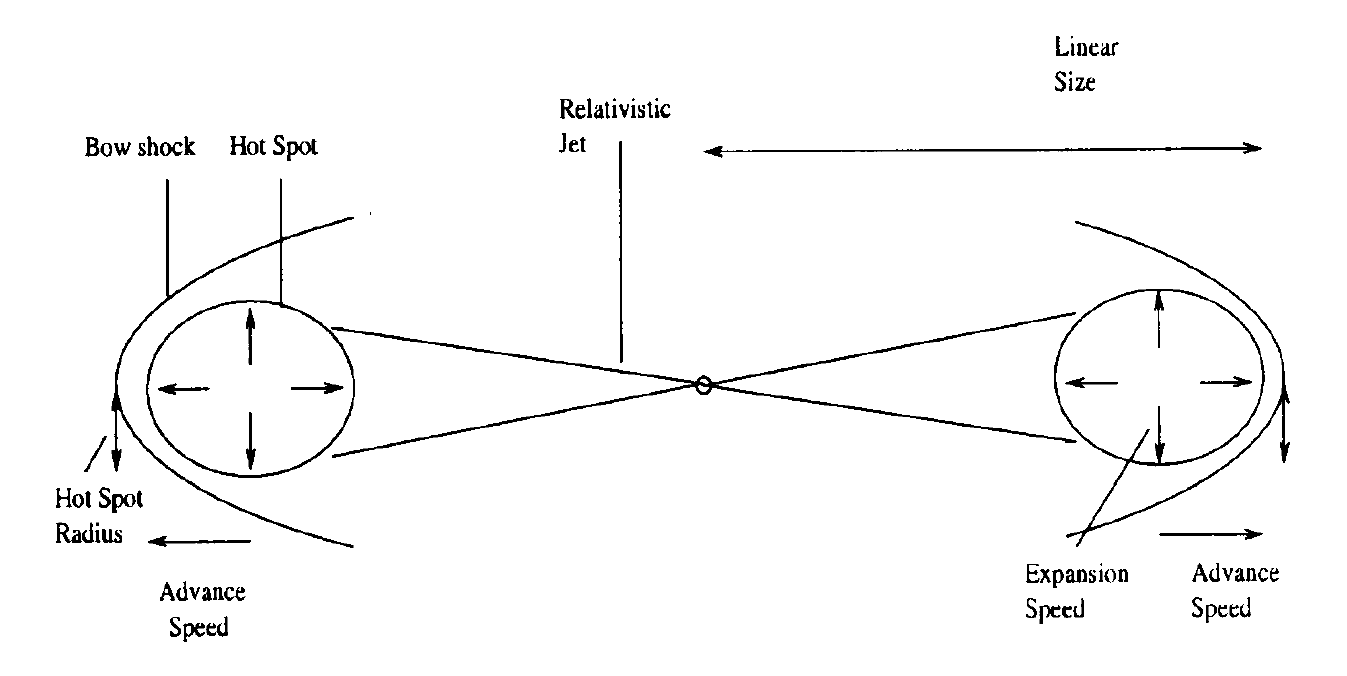
\includegraphics[width=0.5\textwidth]{C:/Users/henri/OneDrive/Documents/NTNU/Semester 10/Masteroppgave/Plots/hot_spot_expansion.png}
    \caption{Schematic of the shock in the CSO. The shock is created by the expansion of the lobes into the ambient medium through jet pressure. Image taken from \cite{Perucho_2002}}
    \label{fig:CSO_shock}
\end{figure}



\subsection{Composition/Mass Loading}
A big problem in determining the viability of UHECRs and neutrino sources is the problem of ion density and composition. The available data obtained through radio measurements or other wavelengths are usually attributed to electrons.

\subsubsection{Stellar Mass Loading}
A mechanism for the deceleration of the jet in both CSO $2.0$ and $2.1$ stages is mass loading. That being the jet encountering various densities that supply an increase of mass to the jet, slowing it down sufficiently. In \cite{sullivan2024smallscale}, they find that the jet needs a mass loading rate of $0.2 M_{\odot} \text{yr}^{-1}$ for $1000$ years in order to decelerate the jet sufficiently to explain the observed CSO $2.1$ lifetimes. This loading rate can allow us to make simple estimates of the ion density that ends up in the lobes and that may experience acceleration.

For a given mass loading rate, one can assume an initial mass composition. By assuming that the mass loading is caused by stellar objects caught by the expanding jet, one can make some estimations. These objects will have a composition similar to the solar composition. The solar composition is $74\%$ hydrogen, $24\%$ helium, and $2\%$ other elements. With this density, one can then estimate the number density of ions in the lobes assuming all mass loading ends up in the lobes via the following formula:

\begin{equation}
    n_{\text{ions}} = \frac{0.2 M_{\odot}\times 1000 \text{yr}}{\frac{4}{3} \pi R_{\text{lobe}}^3 (74\%m_p+24\%m_{\text{helium}}+2\%m_{\text{heavier ions}})}
\end{equation}

Setting $R = 10$ pc, a not unreasonable number for CSO 2.1, we get the number density of ions to be $n_{\text{ions}} = 2.9  \text{cm}^{-3}$. This is not an unreasonably high number for the number density, and it is possible that the ion density is higher than this with part of the jet energy being carried by ions. From this estimate, one also receives the metallicity of the lobes, which is $Z = 0.02$, which is the solar metallicity. This as well is not an unreasonable number but is based on the assumption that the mass loading is caused by stellar objects.

\cite{sullivan2024smallscale} find that the number of stars needed for the...

\subsubsection{Metallicity}
The metallicity of the lobes is also an unknown quantity.

\subsection{Emissivity of the System}
Based on the magnetic field strength, one can estimate the possible maximum energy achieved by a proton. In addition to this, one can estimate the number density of protons in the system through the mass loading rate and a composition by assuming it to be equal to that of solar masses. One also has the density of CSO sources to which this process is happening. With all this information and given a few assumptions on the energy spectra of the protons, one can estimate the emissivity of UHECRs from these sources.

The energy spectrum of protons undergoing first-order acceleration is usually a power law, but commonly one uses a broken power law to describe the spectrum. The spectrum of the number of protons per unit energy is given by:

\begin{equation}
    \label{eq:proton_spectrum}
    N(\gamma) = \begin{cases}
    N_0 \gamma^{-\alpha} & \gamma < \gamma_{\text{break}} \\
    N_0 \gamma_{\text{break}}\gamma^{-\alpha-1} & \gamma > \gamma_{\text{break}}
    \end{cases}
\end{equation}

By arguing that the number of ions in the lobe is equal to the total mass loaded into the lobe, $V_{\text{lobe}} n_{\text{Ion}} = \int_{\gamma_{\text{min}}}^{\gamma_{\text{max}}} N(\gamma) d\gamma$, one can normalize the spectrum. In addition to this, one can separate the number of ions into those of different species by multiplying with the percentage of the mass that is of that species. With this, one can estimate the internal energy of any desired species in the lobe. $\gamma_{\text{max}}$ can then be estimated based on the maximum energy of the particular species. The total internal energy of any species in the lobe can then be calculated as,

\begin{equation}
    U_{\text{Ion}} = m_p c^2 \int_{\gamma_{\text{min}}}^{\gamma_{\text{max}}} \gamma N(\gamma)d\gamma
\end{equation}

By assuming that all internal energy is converted to UHECRs and radiated away at a constant rate, one can estimate the luminosity of cosmic rays as $L_{\text{species}} = U_{\text{species}}/t_{\text{life}}$. One can separate the internal energy stored in all ions to those of the most energetic, that will become UHECRs by calculating the separate internal energy for UHECRs. That is to say, only ions with energy larger than $\gamma > 10^{10}$. By using our estimate of the density of CSO 2.0s at $10^{-5} \text{Mpc}^{-3}$, $\gamma_{\text{max}} = 3 \times 10^{19} \times Z$ and $\gamma_{\text{min}} = 3$, one can estimate the emissivity of UHECRs per species as $Q_{\text{UHECR}} = L_{\text{species}} n_{\text{CSO}}$.

The results of the calculations can be seen in table \ref{tab:emissivity_mass_load}.


 \begin{table}[h!]
    \centering
    \begin{tabular}{|c|c|c|c|}
    \hline
    \textbf{Variable} & \textbf{Protons} & \textbf{Helium} & \textbf{Heavier Ions} \\
    \hline
    \textbf{$u$ (erg cm$^{-3}$)} & \(8.284 \times 10^{-12}\) & \(1.075 \times 10^{-11}\) & \(6.045 \times 10^{-12}\) \\
    \hline
    \textbf{L (erg s$^{-1}$)} & \(1.020 \times 10^{48}\) & \(1.323 \times 10^{48}\) & \(7.440 \times 10^{47}\) \\
    \hline
    \textbf{$\epsilon$ (erg Mpc$^{-3}$ yr$^{-1}$)} & \(3.858 \times 10^{50}\) & \(5.005 \times 10^{50}\) & \(2.815 \times 10^{50}\) \\
    \hline
    \textbf{$u_{\text{UHECRs}}$ (erg cm$^{-3}$ )} & \(4.692 \times 10^{-29}\) & \(6.087 \times 10^{-29}\) & \(3.424 \times 10^{-29}\) \\
    \hline
    \textbf{$L_{\text{UHECRs}}$ (erg s$^{-1}$)} & \(5.774 \times 10^{30}\) & \(7.491 \times 10^{30}\) & \(4.214 \times 10^{30}\) \\
    \hline
    \textbf{$\epsilon_{\text{UHECRs}}$  (erg Mpc$^{-3}$ yr$^{-1}$)} & \(2.185 \times 10^{33}\) & \(2.835 \times 10^{33}\) & \(1.595 \times 10^{33}\) \\
    \hline
    \end{tabular}
    \caption{Mass Loading and Extra-Galactic Results for Different Species}
    \label{tab:emissivity_mass_load}
    \end{table}
 


\subsection{Neutrino Emissivity}
